% This is "sig-alternate.tex" V2.1 April 2013
% This file should be compiled with V2.5 of "sig-alternate.cls" May 2012
%
% This example file demonstrates the use of the 'sig-alternate.cls'
% V2.5 LaTeX2e document class file. It is for those submitting
% articles to ACM Conference Proceedings WHO DO NOT WISH TO
% STRICTLY ADHERE TO THE SIGS (PUBS-BOARD-ENDORSED) STYLE.
% The 'sig-alternate.cls' file will produce a similar-looking,
% albeit, 'tighter' paper resulting in, invariably, fewer pages.
%
% ----------------------------------------------------------------------------------------------------------------
% This .tex file (and associated .cls V2.5) produces:
%       1) The Permission Statement
%       2) The Conference (location) Info information
%       3) The Copyright Line with ACM data
%       4) NO page numbers
%
% as against the acm_proc_article-sp.cls file which
% DOES NOT produce 1) thru' 3) above.
%
% Using 'sig-alternate.cls' you have control, however, from within
% the source .tex file, over both the CopyrightYear
% (defaulted to 200X) and the ACM Copyright Data
% (defaulted to X-XXXXX-XX-X/XX/XX).
% e.g.
% \CopyrightYear{2007} will cause 2007 to appear in the copyright line.
% \crdata{0-12345-67-8/90/12} will cause 0-12345-67-8/90/12 to appear in the copyright line.
%
% ---------------------------------------------------------------------------------------------------------------
% This .tex source is an example which *does* use
% the .bib file (from which the .bbl file % is produced).
% REMEMBER HOWEVER: After having produced the .bbl file,
% and prior to final submission, you *NEED* to 'insert'
% your .bbl file into your source .tex file so as to provide
% ONE 'self-contained' source file.
%
% ================= IF YOU HAVE QUESTIONS =======================
% Questions regarding the SIGS styles, SIGS policies and
% procedures, Conferences etc. should be sent to
% Adrienne Griscti (griscti@acm.org)
%
% Technical questions _only_ to
% Gerald Murray (murray@hq.acm.org)
% ===============================================================
%
% For tracking purposes - this is V2.0 - May 2012

\documentclass{sig-alternate-05-2015}
\usepackage[lined,linesnumbered,boxed,vlined,ruled]{algorithm2e}
\usepackage{graphicx,epsfig,subfigure}
\usepackage{xspace}
\usepackage[mathscr]{eucal}
\usepackage[nospace]{cite}
\usepackage{amsfonts}
\usepackage{amsmath}
\usepackage{amssymb}
\usepackage{enumitem}
\usepackage{tikz}
\usepackage{graphicx}
\usepackage{hyperref}
\usepackage{multirow}
\usepackage{subfigure}
\usetikzlibrary{decorations.pathreplacing}
\usetikzlibrary{matrix}
\usetikzlibrary{positioning}
\usetikzlibrary{patterns}

\DeclareMathOperator*{\argmin}{arg\,min}

\usepackage{CJK}
\usepackage[top=2cm, bottom=2cm, left=2cm, right=2cm]{geometry}
\usepackage{algorithm}
\usepackage{algorithmicx}
\usepackage{algpseudocode}
 
\floatname{algorithm}{算法}
\renewcommand{\algorithmicrequire}{\textbf{输入:}}
\renewcommand{\algorithmicensure}{\textbf{输出:}}

\begin{document}

% Copyright
\setcopyright{acmcopyright}
%\setcopyright{acmlicensed}
%\setcopyright{rightsretained}
%\setcopyright{usgov}
%\setcopyright{usgovmixed}
%\setcopyright{cagov}
%\setcopyright{cagovmixed}


% DOI
\doi{10.475/123_4}

% ISBN
\isbn{123-4567-24-567/08/06}

%Conference
\conferenceinfo{PLDI '13}{June 16--19, 2013, Seattle, WA, USA}

\acmPrice{\$15.00}

%
% --- Author Metadata here ---
\conferenceinfo{WOODSTOCK}{'97 El Paso, Texas USA}
%\CopyrightYear{2007} % Allows default copyright year (20XX) to be over-ridden - IF NEED BE.
%\crdata{0-12345-67-8/90/01}  % Allows default copyright data (0-89791-88-6/97/05) to be over-ridden - IF NEED BE.
% --- End of Author Metadata ---

\title{{\ttlit ACM} My First Paper 
Format\titlenote{(Produces the permission block, and
copyright information). For use with
SIG-ALTERNATE.CLS. Supported by ACM.}}
\subtitle{[Extended Abstract]
\titlenote{A full version of this paper is available as
\textit{Author's Guide to Preparing ACM SIG Proceedings Using
\LaTeX$2_\epsilon$\ and BibTeX} at
\texttt{www.acm.org/eaddress.htm}}}
%
% You need the command \numberofauthors to handle the 'placement
% and alignment' of the authors beneath the title.
%
% For aesthetic reasons, we recommend 'three authors at a time'
% i.e. three 'name/affiliation blocks' be placed beneath the title.
%
% NOTE: You are NOT restricted in how many 'rows' of
% "name/affiliations" may appear. We just ask that you restrict
% the number of 'columns' to three.
%
% Because of the available 'opening page real-estate'
% we ask you to refrain from putting more than six authors
% (two rows with three columns) beneath the article title.
% More than six makes the first-page appear very cluttered indeed.
%
% Use the \alignauthor commands to handle the names
% and affiliations for an 'aesthetic maximum' of six authors.
% Add names, affiliations, addresses for
% the seventh etc. author(s) as the argument for the
% \additionalauthors command.
% These 'additional authors' will be output/set for you
% without further effort on your part as the last section in
% the body of your article BEFORE References or any Appendices.

\numberofauthors{8} %  in this sample file, there are a *total*
% of EIGHT authors. SIX appear on the 'first-page' (for formatting
% reasons) and the remaining two appear in the \additionalauthors section.
%
\author{
% You can go ahead and credit any number of authors here,
% e.g. one 'row of three' or two rows (consisting of one row of three
% and a second row of one, two or three).
%
% The command \alignauthor (no curly braces needed) should
% precede each author name, affiliation/snail-mail address and
% e-mail address. Additionally, tag each line of
% affiliation/address with \affaddr, and tag the
% e-mail address with \email.
%
% 1st. author
\alignauthor
Ben Trovato\titlenote{Dr.~Trovato insisted his name be first.}\\
       \affaddr{Institute for Clarity in Documentation}\\
       \affaddr{1932 Wallamaloo Lane}\\
       \affaddr{Wallamaloo, New Zealand}\\
       \email{trovato@corporation.com}
% 2nd. author
\alignauthor
G.K.M. Tobin\titlenote{The secretary disavows
any knowledge of this author's actions.}\\
       \affaddr{Institute for Clarity in Documentation}\\
       \affaddr{P.O. Box 1212}\\
       \affaddr{Dublin, Ohio 43017-6221}\\
       \email{webmaster@marysville-ohio.com}
% 3rd. author
\alignauthor Lars Th{\o}rv{\"a}ld\titlenote{This author is the
one who did all the really hard work.}\\
       \affaddr{The Th{\o}rv{\"a}ld Group}\\
       \affaddr{1 Th{\o}rv{\"a}ld Circle}\\
       \affaddr{Hekla, Iceland}\\
       \email{larst@affiliation.org}
%\and  % use '\and' if you need 'another row' of author names
% 4th. author
%\alignauthor Lawrence P. Leipuner\\
%       \affaddr{Brookhaven Laboratories}\\
%       \affaddr{Brookhaven National Lab}\\
%       \affaddr{P.O. Box 5000}\\
%       \email{lleipuner@researchlabs.org}
%% 5th. author
%\alignauthor Sean Fogarty\\
%       \affaddr{NASA Ames Research Center}\\
%       \affaddr{Moffett Field}\\
%       \affaddr{California 94035}\\
%       \email{fogartys@amesres.org}
%% 6th. author
%\alignauthor Charles Palmer\\
%       \affaddr{Palmer Research Laboratories}\\
%       \affaddr{8600 Datapoint Drive}\\
%       \affaddr{San Antonio, Texas 78229}\\
%       \email{cpalmer@prl.com}
}
% There's nothing stopping you putting the seventh, eighth, etc.
% author on the opening page (as the 'third row') but we ask,
% for aesthetic reasons that you place these 'additional authors'
% in the \additional authors block, viz.
\additionalauthors{Additional authors: John Smith (The Th{\o}rv{\"a}ld Group,
email: {\texttt{jsmith@affiliation.org}}) and Julius P.~Kumquat
(The Kumquat Consortium, email: {\texttt{jpkumquat@consortium.net}}).}
\date{30 July 1999}
% Just remember to make sure that the TOTAL number of authors
% is the number that will appear on the first page PLUS the
% number that will appear in the \additionalauthors section.

\maketitle
\begin{abstract}
As is widely known, the electronic are closely connected to the economic development. Lots of work has been placed on the regression relationship between the economic metrics and electricity-related indexes, which not focus on the tendency wholly. Obviously, the economic and electricity data can be treated as trajectories composed of points with 
\end{abstract}


%
% The code below should be generated by the tool at
% http://dl.acm.org/ccs.cfm
% Please copy and paste the code instead of the example below. 
%
%\begin{CCSXML}
%<ccs2012>
% <concept>
%  <concept_id>10010520.10010553.10010562</concept_id>
%  <concept_desc>Computer systems organization~Embedded systems</concept_desc>
%  <concept_significance>500</concept_significance>
% </concept>
% <concept>
%  <concept_id>10010520.10010575.10010755</concept_id>
%  <concept_desc>Computer systems organization~Redundancy</concept_desc>
%  <concept_significance>300</concept_significance>
% </concept>
% <concept>
%  <concept_id>10010520.10010553.10010554</concept_id>
%  <concept_desc>Computer systems organization~Robotics</concept_desc>
%  <concept_significance>100</concept_significance>
% </concept>
% <concept>
%  <concept_id>10003033.10003083.10003095</concept_id>
%  <concept_desc>Networks~Network reliability</concept_desc>
%  <concept_significance>100</concept_significance>
% </concept>
%</ccs2012>  
%\end{CCSXML}
%
%\ccsdesc[500]{Computer systems organization~Embedded systems}
%\ccsdesc[300]{Computer systems organization~Redundancy}
%\ccsdesc{Computer systems organization~Robotics}
%\ccsdesc[100]{Networks~Network reliability}


%
% End generated code
%

%
%  Use this command to print the description
%
\printccsdesc

% We no longer use \terms command
%\terms{Theory}

\keywords{Electricity; Trajectory; Similarity; Economic Indicators}

\section{Introduction}
China has gone through a rapid economic growth in the past three decades, and economy boosting in east china area has been always a highlight. Ever since, electricity has been a powerful catalyst for social development and economic growth. Empirically, economic fluctuation would cause changes in electricity consumption and electricity consumption can also reflect the economic change. There has been much interests in the causal relationship between economic growth and electricity consumption using the regression or statistical method. However, though the economic indicators and electricity consumption can be viewed as time series and lots of trajectory similarity methods exist, a big gap still lies midst them. Our work in this paper would focus on the exploit of internal link between economic indicators and electricity consumption using trajectory similarity.

Nowadays, the GDP growth has slower to blew 7\%, which officially is called "new normal". Economic policies would adjust to this new situation, thus asking energy strategies to change. Consequently, the study of the casual relationship between economic indicators and the electricity consumption would shed light on future energy policies, such as the energy conservation, the planning of capacity expansion and the reliable supply of electricity.
  
There are numerous economic indicators and previous work mainly focused on the simple GDP. The study of the relationship between energy consumption and economic growth started with the seminal work of \cite{kraft:relationship}, in which causality between the energy consumption and GNP growth was found using Granger test. Subsequently, actual circumstances in the developed countries was studied like the United Kingdom, Germany, Italy\cite{yu:causal, erol1987causal}. Due to the boosting prosperity, Asian economy also attracted the eyes of researchers like South Korea and Singapore. The cointegration and error-correction models were also applied to research from the viewpoint of the time-series\cite{glasure1998cointegration}.

However, previous work just treat the data as 

Compare to the previous work, our paper has made the following contributions.
\begin{itemize}
	\item We proposed an similarity metrics that 
	\item We focused on specific provinces in the east China.
	\item Quantitive indicators are tested and the most closely connected are sought.
\end{itemize}

The rest part of this paper is organized as follows. We formalize our question in section 2 and introduce our algorithms in section 3. In section 4, we will elaborate our experiments and highlight our contributions. At last, the section 5 will give the conclusion and the future work.

\section{Problem Formulation}
In this section, we will formalize our work into a segement-similarity question and define the notations that we need in the blow.

The time series of economic indicators and electricity consumption would be viewed as a segment. We should evaluate the correlation of economic indicators with electricity consumption through the similarity between the two segments like in Fig 1.[[[[[Here , we should  put one Picture of two examples]]]]] . Before we elaborate the concise similarity problem, we firstly define some relevant notations.
\newcommand{\loci}[1]{\ensuremath{p^{#1}}}
\newdef{definition}{Definition}
\begin{definition}
Suppose we have a series of data in \textit{n} months, each monthly data is composed by \textbf{\{date, val\}}, in which $date$ is the month, and $val$ is the value of economic indicator or electricity consumption. A \textit{segment $T$} is a sequence of data points, i.e.$This place is suspicious$, $T=\{\loci{1}, \loci{2}, \cdots, \loci{|T|}\}$,  where $\loci{k}$ is a data point. And $|T|$ is the number of data points in $T$.
\end{definition}

And then, we would use the area of the polygon enclosed by two segments to evaluate the relevance between the economic indicators and the electricity consumption. Given two segments, it is very obvious to see that the less the enclosed area of these two segments is, the more similar the tendency of these two series is. The area enclosed by two segments is usually calculate by:
\begin{displaymath}
\textbf{S} = \sum_{k=1}^{n-1}\Delta S_k	
\end{displaymath}

Each part of the enclosed polygon \textit{$\Delta S_k$} is that the area of shape enclosed by the two segments and vertical coordinates. According to the different tendencies, we can conclude just two cases.
\begin{itemize}
	\item Two segments doesn't intersect. Then, the enclosed part is a trapezoid, of which area is calculated as:
\begin{equation}
	\Delta S_k = \frac{(a + b) * (t_{k+1} - t_k)}{2}
\end{equation}
	\item Two segments intersects. Then, we can treat it as the sum of two triangles.
\begin{equation}
	\Delta S_k = \frac{a * h_i}{2} + \frac{b * h_j}{2}, h_i + h_j = t_{k+1} - t_k 
\end{equation}
\end{itemize} 

Though we have proposed the area of two segments, it cannot be used to evaluate the similarity of two segments. We want to compare the tendency of two indexes. So, case may be that if two lines goes in the same direction but their distance is very long, we still get the much larger area. So, we can move one of the two lines vertically. With different distances, we would get different area, from which the least area is the most appropriate value to reflect the coincide. So, we could use the notation of MINS as the real area.
\begin{equation}
	MINS = \min{\textbf{S}}	
\end{equation}

Given the statistical report, we could know that different indicators exist the time offset. Given two segments, if we move one of them horizontally, we could get different \textbf{MINS}. Among all the results, the time offset corresponding to the least val is a candidate for the real time offset. Once we got the least similarity for economic indicators, we could rank the similarities of these indicators and found the top-k indicators closely connected to the electricity consumption. We can formalize our problem as one top-k problem as follow:
\begin{definition}
	[[[This part, we can put the top-K problem]]]]
\end{definition} 
\section{Algorithms}
In this section, we describe a novel top-k algorithm based on the area similarity to find the top-k relevant economic indicators. 
\subsection{Similarity}

\begin{CJK*}{UTF8}{gkai}
    \begin{algorithm}
        \caption{用归并排序求逆序数}
        \begin{algorithmic}[1] %每行显示行号
            \Require $Array$Array,$n$数组大小
            \Ensure 逆序数
            \Function {MergerSort}{$Array, left, right$}
                \State $result \gets 0$
                \If {$left < right$}
                    \State $middle \gets (left + right) / 2$
                    \State $result \gets result +$ \Call{MergerSort}{$Array, left, middle$}
                    \State $result \gets result +$ \Call{MergerSort}{$Array, middle, right$}
                    \State $result \gets result +$ \Call{Merger}{$Array,left,middle,right$}
                \EndIf
                \State \Return{$result$}
            \EndFunction
            \State
            \Function{Merger}{$Array, left, middle, right$}
                \State $i\gets left$
                \State $j\gets middle$
                \State $k\gets 0$
                \State $result \gets 0$
                \While{$i<middle$ \textbf{and} $j<right$}
                    \If{$Array[i]<Array[j]$}
                        \State $B[k++]\gets Array[i++]$
                    \Else
                        \State $B[k++] \gets Array[j++]$
                        \State $result \gets result + (middle - i)$
                    \EndIf
                \EndWhile
                \While{$i<middle$}
                    \State $B[k++] \gets Array[i++]$
                \EndWhile
                \While{$j<right$}
                    \State $B[k++] \gets Array[j++]$
                \EndWhile
                \For{$i = 0 \to k-1$}
                    \State $Array[left + i] \gets B[i]$
                \EndFor
                \State \Return{$result$}
            \EndFunction
        \end{algorithmic}
    \end{algorithm}
\end{CJK*}

\subsection{Hysteresis}

\section{Experiments}
\subsection{Data Preprocessing}
Different data source supply data with different dimensions. So, we must normalize the data to make them comparable. 
\section{Conclusion}
\subsection{Figures}

\begin{figure}
\centering
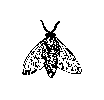
\includegraphics{fly}
\caption{A sample black and white graphic.}
\end{figure}

\begin{figure}
\centering
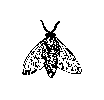
\includegraphics[height=1in, width=1in]{fly}
\caption{A sample black and white graphic
that has been resized with the \texttt{includegraphics} command.}
\end{figure}

\begin{figure*}
\centering
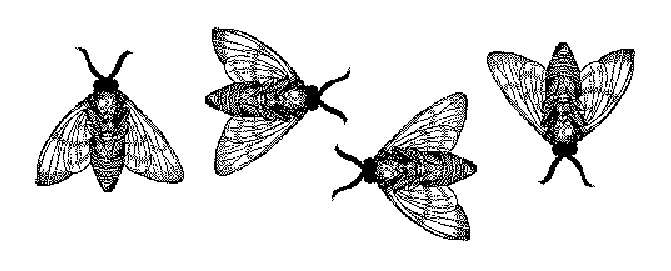
\includegraphics{flies}
\caption{A sample black and white graphic
that needs to span two columns of text.}
\end{figure*}

\begin{figure}
\centering
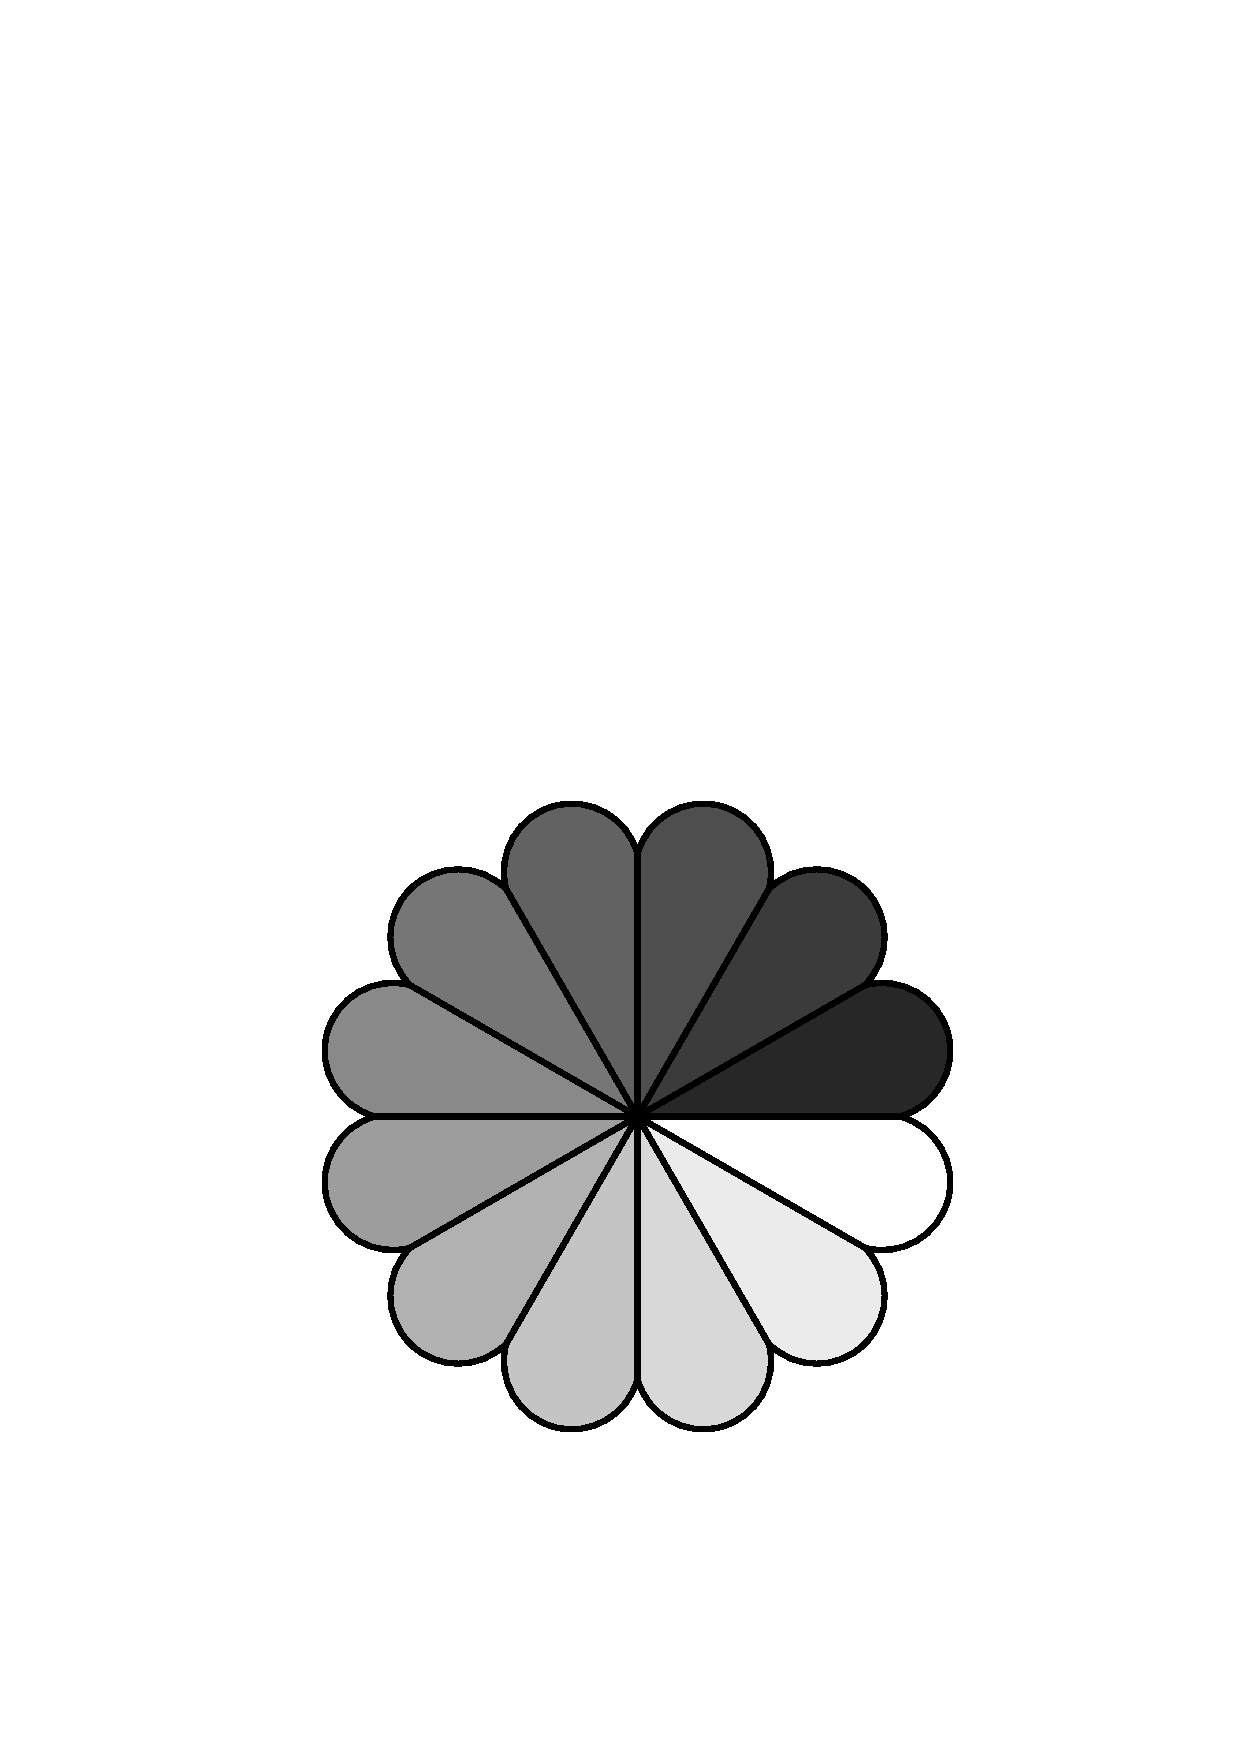
\includegraphics[height=1in, width=1in]{rosette}
\caption{A sample black and white graphic that has
been resized with the \texttt{includegraphics} command.}
\vskip -6pt
\end{figure}

\subsection{Theorem-like Constructs}
Other common constructs that may occur in your article are
the forms for logical constructs like theorems, axioms,
corollaries and proofs.  There are
two forms, one produced by the
command \texttt{{\char'134}newtheorem} and the
other by the command \texttt{{\char'134}newdef}; perhaps
the clearest and easiest way to distinguish them is
to compare the two in the output of this sample document:

This uses the \textbf{theorem} environment, created by
the\linebreak\texttt{{\char'134}newtheorem} command:
\newtheorem{theorem}{Theorem}
\begin{theorem}
Let $f$ be continuous on $[a,b]$.  If $G$ is
an antiderivative for $f$ on $[a,b]$, then
\begin{displaymath}\int^b_af(t)dt = G(b) - G(a).\end{displaymath}
\end{theorem}

The other uses the \textbf{definition} environment, created
by the \texttt{{\char'134}newdef} command:
\begin{definition}
If $z$ is irrational, then by $e^z$ we mean the
unique number which has
logarithm $z$: \begin{displaymath}{\log e^z = z}\end{displaymath}
\end{definition}

Two lists of constructs that use one of these
forms is given in the
\textit{Author's  Guidelines}.
 
There is one other similar construct environment, which is
already set up
for you; i.e. you must \textit{not} use
a \texttt{{\char'134}newdef} command to
create it: the \textbf{proof} environment.  Here
is a example of its use:
\begin{proof}
Suppose on the contrary there exists a real number $L$ such that
\begin{displaymath}
\lim_{x\rightarrow\infty} \frac{f(x)}{g(x)} = L.
\end{displaymath}
Then
\begin{displaymath}
l=\lim_{x\rightarrow c} f(x)
= \lim_{x\rightarrow c}
\left[ g{x} \cdot \frac{f(x)}{g(x)} \right ]
= \lim_{x\rightarrow c} g(x) \cdot \lim_{x\rightarrow c}
\frac{f(x)}{g(x)} = 0\cdot L = 0,
\end{displaymath}
which contradicts our assumption that $l\neq 0$.
\end{proof}

Complete rules about using these environments and using the
two different creation commands are in the
\textit{Author's Guide}; please consult it for more
detailed instructions.  If you need to use another construct,
not listed therein, which you want to have the same
formatting as the Theorem
or the Definition\cite{salas:calculus} shown above,
use the \texttt{{\char'134}newtheorem} or the
\texttt{{\char'134}newdef} command,
respectively, to create it.

%
% The following two commands are all you need in the
% initial runs of your .tex file to
% produce the bibliography for the citations in your paper.
\bibliographystyle{abbrv}
\bibliography{sigproc}  % sigproc.bib is the name of the Bibliography in this case
% You must have a proper ".bib" file
%  and remember to run:
% latex bibtex latex latex
% to resolve all references
%
% ACM needs 'a single self-contained file'!
%
%APPENDICES are optional
%\balancecolumns
\appendix
%Appendix A
\section{Headings in Appendices}
The rules about hierarchical headings discussed above for
the body of the article are different in the appendices.
In the \textbf{appendix} environment, the command
\textbf{section} is used to
indicate the start of each Appendix, with alphabetic order
designation (i.e. the first is A, the second B, etc.) and
a title (if you include one).  So, if you need
hierarchical structure
\textit{within} an Appendix, start with \textbf{subsection} as the
highest level. Here is an outline of the body of this
document in Appendix-appropriate form:
\subsection{Introduction}
\subsection{The Body of the Paper}
\subsubsection{Type Changes and  Special Characters}
\subsubsection{Math Equations}
\paragraph{Inline (In-text) Equations}
\paragraph{Display Equations}
\subsubsection{Citations}
\subsubsection{Tables}
\subsubsection{Figures}
\subsubsection{Theorem-like Constructs}
\subsubsection*{A Caveat for the \TeX\ Expert}
\subsection{Conclusions}
\subsection{Acknowledgments}
\subsection{Additional Authors}
This section is inserted by \LaTeX; you do not insert it.
You just add the names and information in the
\texttt{{\char'134}additionalauthors} command at the start
of the document.
\subsection{References}
Generated by bibtex from your ~.bib file.  Run latex,
then bibtex, then latex twice (to resolve references)
to create the ~.bbl file.  Insert that ~.bbl file into
the .tex source file and comment out
the command \texttt{{\char'134}thebibliography}.
% This next section command marks the start of
% Appendix B, and does not continue the present hierarchy
\section{More Help for the Hardy}
The sig-alternate.cls file itself is chock-full of succinct
and helpful comments.  If you consider yourself a moderately
experienced to expert user of \LaTeX, you may find reading
it useful but please remember not to change it.
%\balancecolumns % GM June 2007
% That's all folks!
\end{document}
